The Hodgkin-Huxley model is a system of nonlinear differential equations that represent action potentials movement through nerve cells by three types of ion current: sodium, potassium, and a leak current. 
Describing the transfer of these ions with a circuit allows for equations that model cells electrical properties \cite{Schwiening2012}. 

\subsection{Model Components and Equations}
\label{subsec:hh_equations}
\begin{minipage}{\linewidth}
    \centering
    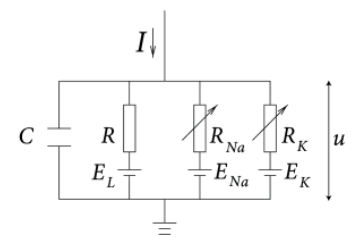
\includegraphics[width=0.8\linewidth]{Figs/ion_circuit.png}
    \captionof{figure}{Circuit representation of ion transfer across the cell membrane \cite{Gerstner2014}}
    \label{fig:ion_circuit}
\end{minipage}

The circuit model represents each component of ion transfer within a nerve cell as an electrical component: 
the ion pumps and the leak channel are represented as resistors; the difference in ion concentration for each ion is represented by a battery; the lipid bilayer is represented by a capacitor \cite{Gerstner2014}.
These components are combined according to the circuit in Figure~\ref{fig:ion_circuit}, to create the equation for current across the cell membrane:
\begin{dmath}
    I = C_{M}\frac{dV}{dt} + \bar{g}_{K}n^4(V - V_{K}) + \bar{g}_{Na}m^3h(V - V_{Na}) + \bar{g}_{l}(V - V_{l})
    \label{eq:ion_current}
\end{dmath}
Relating Equation~\ref{eq:ion_current} to Figure~\ref{fig:ion_circuit}, V is analogous to u, and $V_x$ to $E_x$ (where x represents Na, K, or l). Discerned from the resistance values, $g_x$ (where x is Na, K, or l) represents the maximum conductance of the channel.

\subsection{Gating Variables and Activation/Inactivation}
\label{subsec:gating_variables}

Hodgkins and Huxley theorized that specific ammounts of charged particles would need to move under influence of the membrane potential to allow $Na^+$ or $K^+$ particles to move \cite{Schwiening2012}.
Based on this theory, the model uses three gating variables (m, n, and h) to represent the probability that a channel will be open at a given moment in time. 
For the $Na^+$ channels, m describes the activation of the channel and h is its inactivation. 
Similarly, n describes the activation of the $K^+$ channels.
They found that $n^4$, $m^3$, and h provided a good fit \cite{Schwiening2012}. 
The gating variables are represented across a range of potentials by equations of the form:
\begin{dmath}
    \dot{x} = -\frac{1}{\tau_{x}(u)}[x - x_{0}(u)]
    \label{eq:gating_variables}
\end{dmath}
To interpret Equation~\ref{eq:gating_variables}, let $\dot{x}$ = $\frac{dx}{dt}$ where x stands for m, n, or h. $\tau_0$(u) and $x_0$(u) are conditional variables dependent on the initial membrane potential \cite{Gerstner2014}.
